% ==============================================================================
\section{Módulo de mapeo}
\label{sec:dev_mapeo}
% ==============================================================================

\subsection{Descripción}

El módulo de mapeo mantiene la representación del entorno sobre la que trabajan la
navegación y las alertas, y atiende los requerimientos RF-15, RF-16 y RF-17. El diseño
de TT1 contemplaba una sola retícula de ocupación local. La primera implementación
(\texttt{occupancy\_grid.py}) siguió ese diseño con una retícula fija de
$8 \times 8$~m, pero pronto aparecieron tres problemas. El usuario puede salir de un
área de ocho metros en pocos segundos; una retícula más grande gastaría memoria aunque
casi toda quedara vacía; y el mapa se perdía al apagar el dispositivo. Para resolverlos
se desarrolló el gestor de mapa por bloques (\texttt{map\_manager.py}), que conserva la
misma interfaz de consulta de la retícula original, así que el resto del sistema no tuvo
que cambiar.

\subsection{Mapa global por bloques}

El plano se divide en bloques cuadrados fijos (\emph{chunks}) de $8 \times 8$~m,
anclados al marco de referencia del SLAM. Con celdas de 5~cm, cada bloque tiene
$160 \times 160$ celdas. Los bloques se identifican con un par de índices enteros
$(i, j)$, que pueden ser negativos, y se crean solo cuando un rayo o el propio usuario
llegan a ellos, de modo que el mapa crece únicamente hacia donde se camina. Un punto del
mundo se convierte a su bloque y a su celda local así.

\[
(g_x, g_y) = \left(\left\lfloor \frac{x}{0.05} \right\rfloor,
                   \left\lfloor \frac{y}{0.05} \right\rfloor\right),
\qquad
(i, j) = \left(\left\lfloor \frac{g_x}{160} \right\rfloor,
               \left\lfloor \frac{g_y}{160} \right\rfloor\right),
\qquad
(l_x, l_y) = (g_x - 160\,i,\; g_y - 160\,j)
\]

La idea se parece a los submapas de sistemas como Cartographer
\cite{hess2016cartographer}, con la diferencia de que aquí los bloques tienen una
posición fija en el mundo y no se reacomodan por optimización. Eso mantiene el costo
bajo, a cambio de no corregir la deriva acumulada.

Cada bloque (\texttt{MapChunk}) guarda una matriz de log-odds en punto flotante de
32 bits, que ocupa 100~KB en memoria, y una matriz de impactos de peligros de piso en
enteros de 8 bits, de 25~KB. Guarda también la etiqueta del cuarto al que pertenece, el
número de visitas, las fechas de creación y de última visita, y una bandera que indica
si tiene cambios sin guardar.

Para no llenar la memoria de la Raspberry Pi, se mantienen como máximo 25 bloques
cargados. Si se pasa de ese número, los bloques más alejados del actual (en distancia de
Chebyshev) se guardan en disco y se descargan, y si se vuelven a necesitar se cargan de
nuevo sin que el resto del sistema lo note. Los rayos cruzan de un bloque a otro sin
cortes, porque cada celda se resuelve a su bloque en el momento de leerla o escribirla,
con un pequeño caché del último bloque consultado.

\subsection{Persistencia y re-localización}

Cada mapa se guarda en una carpeta con la siguiente estructura.

\begin{verbatim}
maps/<nombre>/
    chunk_0_0.npz      log-odds (float16) + peligros + metadatos del bloque
    chunk_0_-1.npz     ...
    meta.json          resolución, tamaño de bloque, cuartos etiquetados
    landmarks.json     landmarks confirmados del SLAM (posición, etiqueta,
                       número de avistamientos)
\end{verbatim}

Los bloques se guardan comprimidos y con el log-odds en 16 bits, así que en los mapas
reales ocupan entre 1 y 7~KB cada uno y el recorrido más grande (13 bloques y
26 \emph{landmarks}) ocupa unos 60~KB. Al abrir un mapa se revisa que su resolución y
tamaño de bloque coincidan con la configuración actual, para no mezclar geometrías
distintas. Cuando el sistema arranca en un lugar ya mapeado, se restauran los bloques y
los \emph{landmarks}, y estos últimos se cargan en el SLAM para que el filtro pueda
corregir la pose contra objetos conocidos desde el primer ciclo.

El SLAM siempre arranca en el origen de su propio marco de referencia, así que la
re-localización funciona cuando el usuario empieza la sesión en el mismo punto y mirando
hacia el mismo lado que cuando se creó el mapa, por ejemplo en la entrada de su casa u
oficina. Una primera versión anunciaba como ``zona conocida'' cualquier bloque guardado
aunque el usuario estuviera en otro lugar. Ahora, mientras la re-localización está
pendiente, todos los bloques se reportan como nuevos y no se adoptan las etiquetas de
cuarto; se da por confirmada cuando el EKF acumula tres correcciones contra los
\emph{landmarks} cargados, y en ese momento el sistema lo dice en voz alta.

\subsection{Eventos de cambio de zona}

En cada ciclo el gestor recibe la pose y genera eventos que la interacción puede
anunciar por voz. El evento \texttt{chunk\_change} indica que el usuario entró a otro
bloque y si esa zona ya era conocida o es nueva. El evento \texttt{door\_crossed} se
dispara cuando el usuario pasa a menos de 0.7~m de un \emph{landmark} confirmado de tipo
puerta, lo cual se interpreta como el paso a otro cuarto, con una espera de 60 ciclos
para no repetirlo. Y \texttt{room\_recognized} indica que el bloque al que entró el
usuario tiene una etiqueta de cuarto guardada, como ``cocina''. Los cuartos se numeran
solos al cruzar puertas y se pueden renombrar con una etiqueta propia, que queda en
\texttt{meta.json}.

\subsection{Despeje de la huella del usuario}

Al procesar los videos se vio que, en pasillos sin objetos de las clases que reconoce la
visión, el mapa no registraba espacio libre, porque sin ultrasonido no había rayos que lo
despejaran, y la navegación no encontraba por dónde avanzar. Como el usuario sí pasó por
ahí, en cada ciclo se marca como libre un disco de 0.45~m de radio alrededor de su
posición (\texttt{clearFootprint}). Las celdas que ya superan el umbral de ocupación no
se tocan, para no borrar obstáculos reales.

\subsection{Capa de peligros de piso}

Un hoyo, una coladera, un charco o una escalera hacia abajo no devuelven eco ni detienen
un rayo, porque el espacio de arriba está libre, y aun así no se pueden pisar. Por eso
van en una capa separada del log-odds, siguiendo la idea de los mapas de costo por capas
\cite{lu2014layered}. Las detecciones vienen de la segmentación del módulo de visión
(SegFormer entrenado en ADE20K \cite{xie2021segformer, zhou2017ade20k}) y su distancia se
calcula por proyección al plano del piso. Cada avistamiento suma un impacto a su celda, y
la celda cuenta como peligrosa a partir de dos impactos, así que un parpadeo de la
segmentación no inventa un hoyo. En las consultas, una celda peligrosa se trata como
bloqueada y la navegación la rodea igual que a una pared.

Los impactos también pueden bajar. En cada cuadro, el módulo de visión revisa nueve
columnas de la máscara de piso transitable y, para cada una, mide hasta dónde llega el
piso sin interrupción; con eso arma unos rayos de ``piso libre'' que entrega al mapa
(\texttt{tomarPisoLibre}). Estos rayos no tocan el log-odds, solo le restan un impacto a
cada celda de peligro que cruzan. Así, si la segmentación confundió una mancha con un
hoyo y después la misma zona se ve como piso, el falso peligro se borra en pocos
cuadros. Como su distancia viene de la proyección al piso, se tratan como rango
impreciso y solo recorren la parte cercana del tramo, de modo que no borran un hoyo real
que esté justo donde termina el piso visible.

\subsection{Salida hacia el módulo de navegación}

En cada ciclo, la función \texttt{buildNavigationFrame} junta en una sola estructura, el
cuadro de navegación, todo lo que necesita el módulo de navegación. Sus campos se
describen en la Tabla~\ref{tab:nav_frame}.

\begin{table}[H]
\centering
\caption{Contenido del cuadro de navegación generado por el módulo de mapeo}
\label{tab:nav_frame}
\renewcommand{\arraystretch}{1.25}
\begin{tabular}{|p{4.2cm}|p{10.3cm}|}
\hline
\textbf{Campo} & \textbf{Descripción} \\
\hline
Salida del SLAM & Pose, covarianza, confianza y marca de tiempo. \\
\hline
Mapa local & Parche centrado en el usuario de $4 \times 4$~m ($81 \times 81$ celdas)
con dos canales, la probabilidad de ocupación y los peligros de piso. Las celdas
desconocidas valen 0.5 en el primer canal. \\
\hline
$d_{\text{front}}$, $d_{\text{left}}$, $d_{\text{right}}$ & Distancia libre por sector,
obtenida con los rayos de consulta (Sección~\ref{sec:dev_ray}). \\
\hline
$r_{\text{front}}$, $r_{\text{left}}$, $r_{\text{right}}$ & Nivel de riesgo de 0 a 3
por sector, según la tabla de riesgo de TT1, calculado con las detecciones del ciclo a
menos de 3~m. \\
\hline
Lecturas ultrasónicas & Lecturas de los dos MB1232 ya validadas y sin ecos de piso. \\
\hline
Detecciones y \emph{landmarks} & Detecciones del ciclo y \emph{landmarks}
etiquetados del mapa, que sirven para resolver destinos como ``la salida''. \\
\hline
Bloque y cuarto & Índice del bloque actual y etiqueta del cuarto, si la hay. \\
\hline
\end{tabular}
\end{table}

La Figura~\ref{fig:mapeo_costmap} muestra un ejemplo del mapa local. Para que se viera
el segundo canal, en esta figura se agregó a mano un peligro de piso de
$25 \times 25$~cm delante del usuario.

\begin{figure}[H]
    \centering
    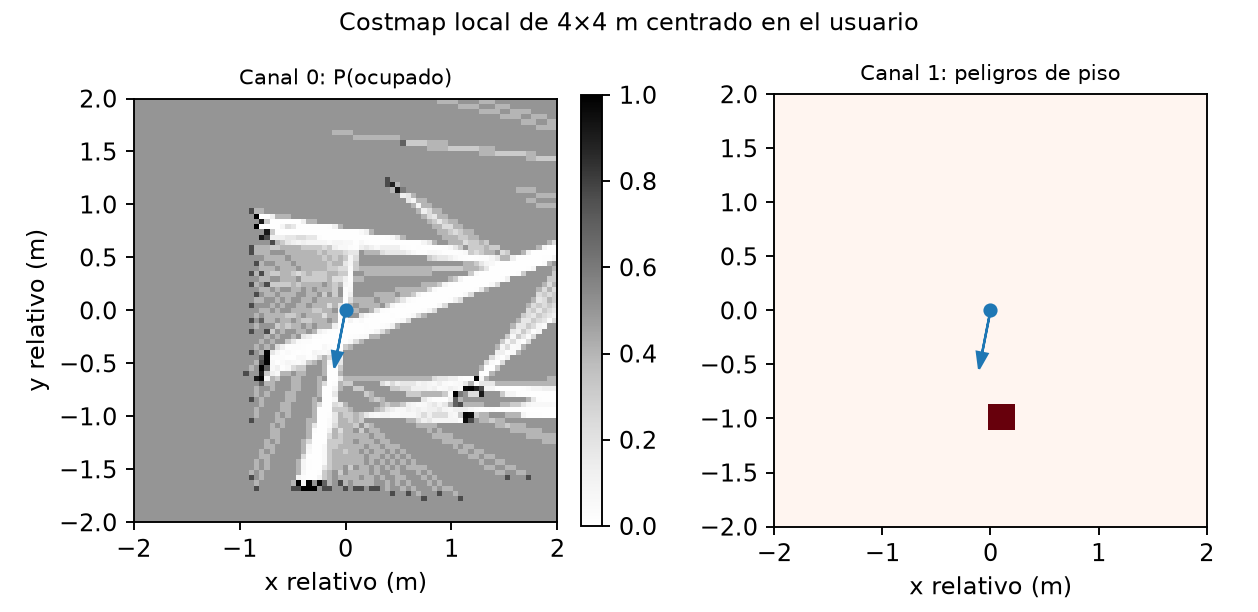
\includegraphics[width=0.85\textwidth]{Capturas_TT2/mapeo_costmap.png}
    \caption{Mapa local de $4 \times 4$~m centrado en el usuario, con la probabilidad de
    ocupación (izquierda) y los peligros de piso (derecha).}
    \label{fig:mapeo_costmap}
\end{figure}

\subsection{Del video al mapa}

Para tener mapas de muchos lugares reales sin recorrerlos todos con el prototipo se
desarrolló el script \texttt{video\_a\_mapa.py}. El script procesa videos grabados en
primera persona con el mismo flujo del sistema (visión, SLAM, Ray Casting y mapa por
bloques) y guarda el resultado. Al final genera un reporte que dice si el mapa tiene
suficiente espacio libre para usarse en el entrenamiento de la navegación y, si no,
sugiere grabar más pasadas por el mismo lugar. También trae recomendaciones de grabación,
como sostener el teléfono a la altura del pecho, caminar y girar despacio porque el giro
se estima con flujo óptico, evitar contraluces y pasar dos o más veces por cada zona
para que los \emph{landmarks} se confirmen.

\subsection{Resultados}

\textbf{Mapas con el prototipo.} \TODO{mapas construidos con el prototipo en recorridos
reales (figura y tabla con bloques, \emph{landmarks}, puertas y superficie libre), y
comparación con un plano o croquis del lugar}.

\textbf{Construcción incremental.} La Figura~\ref{fig:mapeo_evolucion} muestra cómo
evoluciona el mapa del cuarto simulado. El mapa se construye sin información previa
(RF-15); al principio solo se conocen las zonas que alcanzaron los primeros rayos y, al
terminar el recorrido, ya se distinguen el espacio libre, los obstáculos y las paredes
hacia las que el usuario caminó (RF-16). Como los dos ultrasónicos miran al frente con un
haz angosto, las paredes que solo quedan a los costados del recorrido casi no se
registran y buena parte del contorno del cuarto se queda en gris, es decir, sin conocer.

\begin{figure}[H]
    \centering
    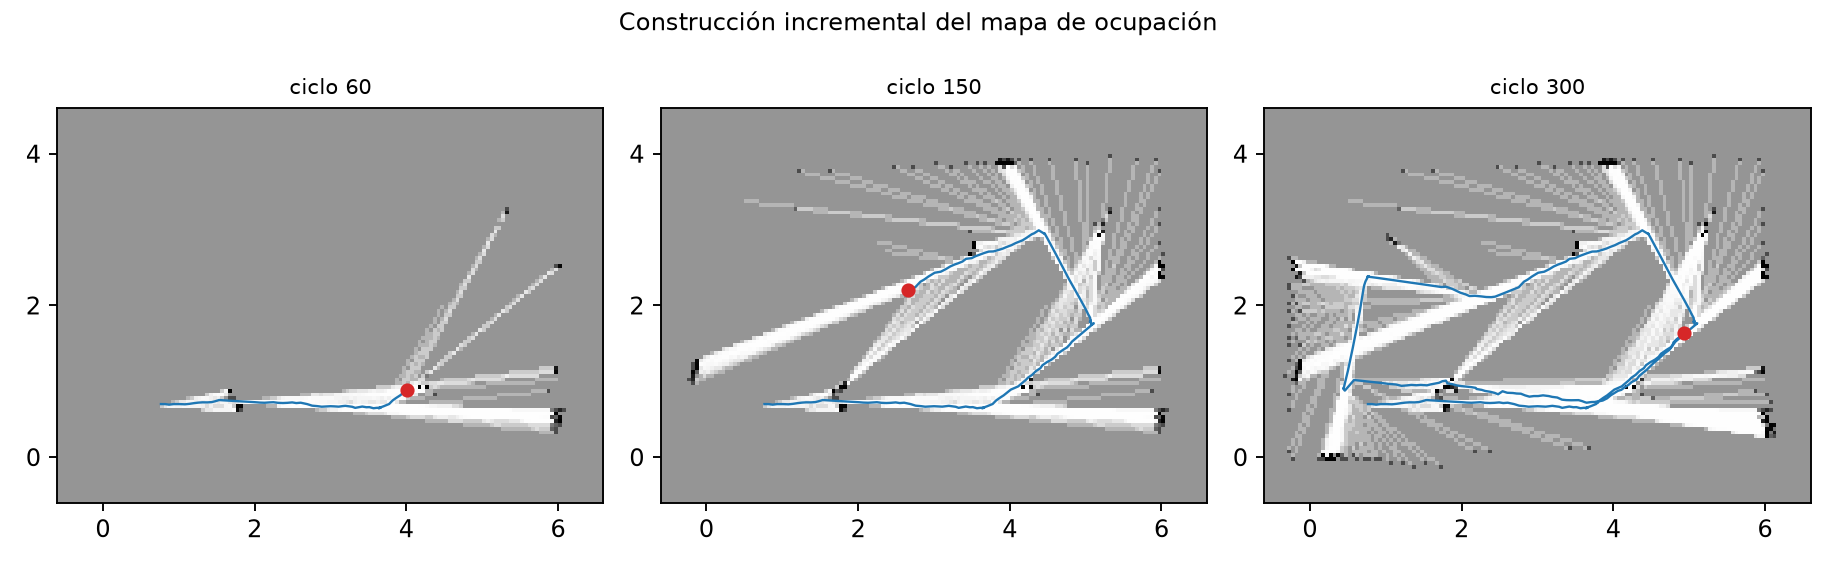
\includegraphics[width=\textwidth]{Capturas_TT2/mapeo_evolucion.png}
    \caption{Mapa de ocupación del cuarto simulado en los ciclos 60, 150 y 300. En blanco
    lo libre, en negro lo ocupado y en gris lo desconocido; la línea azul es la
    trayectoria estimada.}
    \label{fig:mapeo_evolucion}
\end{figure}

\textbf{Aporte del ultrasonido.} El banco de simulación usa el mismo montaje que el
prototipo, con dos sensores frontales paralelos separados 10~cm. Para ver qué tan buena
fue esa decisión se comparó contra otras dos disposiciones y contra el caso sin
ultrasonido (Tabla~\ref{tab:mapeo_us}). La configuración de tres sensores es la que usaba
el banco en una versión anterior, y la de sensores laterales es la que sugería la
descripción electrónica de TT1.

\begin{table}[H]
\centering
\caption{Efecto de la configuración ultrasónica (promedio de seis corridas)}
\label{tab:mapeo_us}
\renewcommand{\arraystretch}{1.2}
\begin{tabular}{|p{6.2cm}|c|c|c|}
\hline
\textbf{Configuración} & \textbf{ATE (m)} & \textbf{Precisión} &
\textbf{Exhaustividad} \\
\hline
Dos sensores frontales, como el prototipo & 0.21 & 0.60 & 0.31 \\
Tres sensores ($0^\circ$, $\pm 40^\circ$) & 0.27 & 0.48 & 0.43 \\
Dos sensores laterales ($\pm 90^\circ$) & 0.28 & 0.55 & 0.48 \\
Sin ultrasonido & 0.30 & 0.60 & 0.05 \\
\hline
\end{tabular}
\end{table}

El montaje del prototipo da la mejor localización (0.21~m) y la mejor precisión del mapa,
porque los ecos frontales coinciden con lo que ve la cámara y las paredes quedan bien
ubicadas. A cambio, registra menos superficie que las configuraciones con sensores
abiertos hacia los lados, con una exhaustividad de 0.31 contra 0.43 a 0.48. Sin
ultrasonido la exhaustividad se desploma a 0.05, porque el mapa solo registra los objetos
anclados a \emph{landmarks} y casi ninguna pared, y su precisión es alta nada más porque
marca muy pocas celdas. El resultado justifica los MB1232 sobre todo por el mapa. Abrir
un poco cada sensor hacia afuera, algo que \texttt{montaje.py} ya permite, podría
recuperar parte de la cobertura lateral, aunque se perdería el traslape central que hace
posible el cálculo estéreo del lado.

\textbf{Mapas de recorridos en video.} La Tabla~\ref{tab:mapeo_reales} resume los mapas
de los 19 videos, y las Figuras~\ref{fig:mapeo_real_pasillo} a
\ref{fig:mapeo_real_banqueta} muestran tres de ellos. Los videos no traen ultrasonido,
así que el espacio libre sale sobre todo de la huella del usuario y las celdas ocupadas
solo de los objetos anclados a \emph{landmarks}.

\begin{table}[H]
\centering
\caption{Mapas generados a partir de videos reales}
\label{tab:mapeo_reales}
\renewcommand{\arraystretch}{1.2}
\begin{tabular}{|l|c|c|c|c|c|}
\hline
\textbf{Recorrido} & \textbf{Bloques} & \textbf{Landmarks} & \textbf{Puertas} &
\textbf{Peligros} & \textbf{Libre observado (m$^2$)} \\
\hline
Calle 1 & 5 & 1 & 0 & 0 & 12.4 \\
Calle 2 & 5 & 5 & 0 & 1 & 10.6 \\
Casa & 6 & 29 & 5 & 11 & 34.5 \\
Pasillo & 9 & 25 & 13 & 1 & 45.4 \\
Plaza comercial & 13 & 26 & 6 & 4 & 38.5 \\
Oficina 1 & 8 & 23 & 11 & 1 & 19.3 \\
Oficina 2 & 4 & 12 & 9 & 0 & 20.4 \\
Video vertical & 5 & 8 & 1 & 5 & 12.7 \\
Oficina 3 & 8 & 28 & 12 & 2 & 16.9 \\
Oficina 4 & 5 & 39 & 17 & 3 & 18.3 \\
Puesto callejero & 4 & 5 & 0 & 2 & 4.2 \\
Banqueta 1 & 5 & 9 & 0 & 8 & 8.1 \\
Avenida 1 & 7 & 8 & 0 & 4 & 13.3 \\
Avenida 2 & 7 & 11 & 0 & 4 & 16.1 \\
Banqueta 2 & 8 & 16 & 0 & 13 & 37.5 \\
Esquina & 5 & 14 & 0 & 7 & 14.0 \\
Sala de maestros 1 & 4 & 4 & 2 & 0 & 1.1 \\
Sala de maestros 2 & 4 & 6 & 5 & 0 & 4.2 \\
Sala de maestros 3 & 4 & 9 & 3 & 0 & 11.5 \\
\hline
\end{tabular}
\end{table}

\begin{figure}[H]
    \centering
    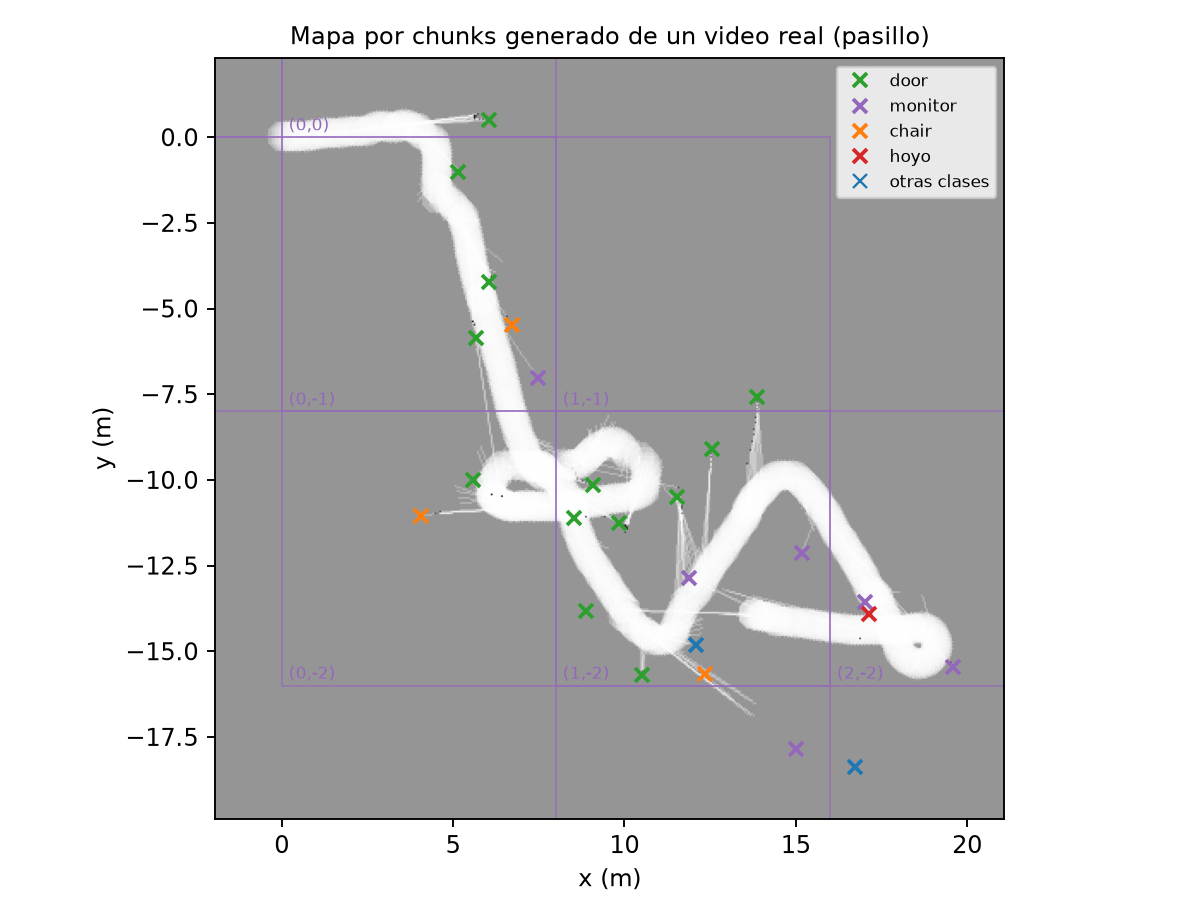
\includegraphics[width=0.8\textwidth]{Capturas_TT2/mapeo_real_pasillo.png}
    \caption{Mapa por bloques del recorrido de un pasillo. Los recuadros morados son los
    bloques de $8 \times 8$~m y las cruces, los \emph{landmarks} por clase.}
    \label{fig:mapeo_real_pasillo}
\end{figure}

\begin{figure}[H]
    \centering
    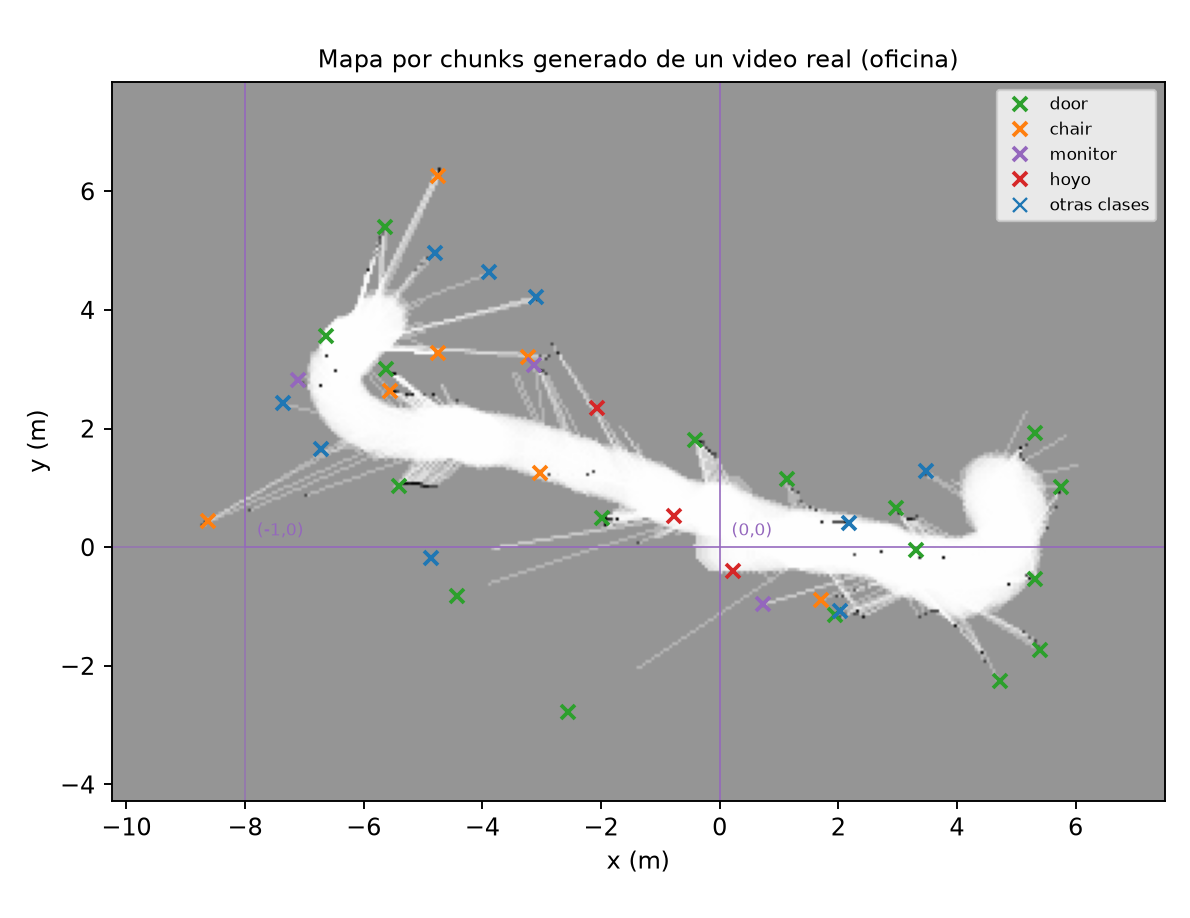
\includegraphics[width=0.8\textwidth]{Capturas_TT2/mapeo_real_oficina.png}
    \caption{Mapa por bloques del recorrido de una oficina.}
    \label{fig:mapeo_real_oficina}
\end{figure}

\begin{figure}[H]
    \centering
    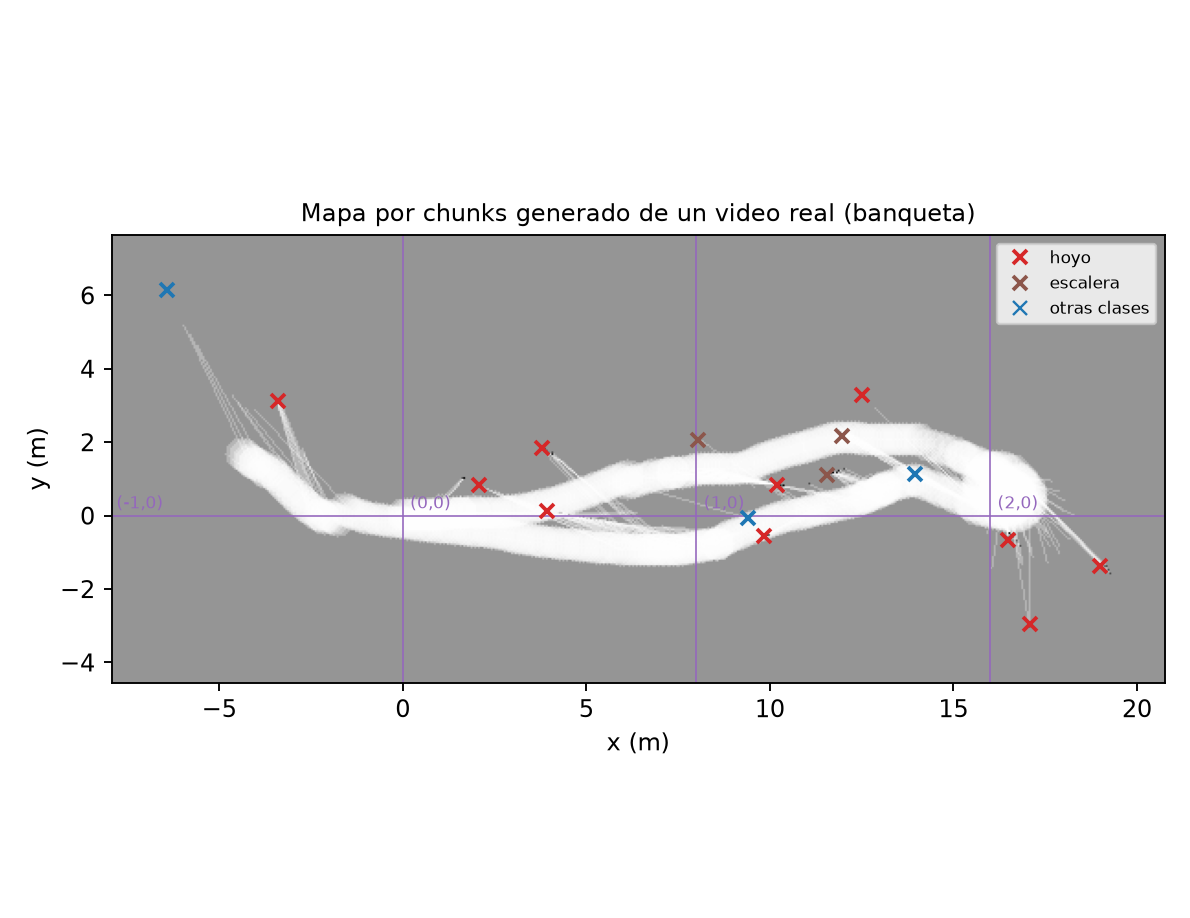
\includegraphics[width=0.8\textwidth]{Capturas_TT2/mapeo_real_banqueta.png}
    \caption{Mapa por bloques del recorrido de una banqueta, con muchos peligros de piso
    registrados.}
    \label{fig:mapeo_real_banqueta}
\end{figure}

En los recorridos de interiores las puertas son la clase más frecuente, lo cual viene
bien porque son los destinos naturales de la navegación (``llévame a la salida''). La
tabla también deja ver falsos positivos, ya que en las oficinas aparecen peligros de piso
que no son hoyos reales, probablemente porque la segmentación confunde reflejos o
cambios de textura del piso con zonas no transitables. Los mapas de calle tienen pocos
\emph{landmarks}, porque hay pocos objetos estáticos de las clases detectables, y en
cambio juntan muchos peligros de piso. En las banquetas, esos peligros pueden ser
escalones y desniveles reales que la segmentación toma por escaleras, o grietas y
manchas del pavimento; con estos datos no hay forma de separarlos.

\textbf{Persistencia.} Los 19 mapas se cargan desde disco con sus bloques,
\emph{landmarks} y valores de log-odds, y se consultan con la misma interfaz que un mapa
en memoria. Las pruebas automatizadas comprueban además que, al guardar y volver a cargar
un mapa, se conservan las celdas ocupadas, los peligros y las etiquetas de cuarto, que los
\emph{landmarks} vuelven al SLAM, que un mapa con geometría distinta se rechaza y que
descargar bloques por falta de memoria no pierde información.

\subsection{Limitaciones}

Los bloques están fijos en el mundo y no se corrigen cuando el SLAM acumula deriva, así
que un error de pose se queda ``congelado'' en el mapa. La re-localización entre
sesiones, por su parte, requiere empezar en el mismo punto y con la misma orientación
con que se creó el mapa. Los peligros de piso solo se borran cuando la cámara vuelve a
ver la zona como piso, así que un falso hoyo que quedó atrás del usuario permanece en el
mapa hasta que regrese por ahí. Los mapas de recorridos en video de la tabla anterior se
construyeron antes de agregar los rayos de piso libre, por lo que sus conteos de
peligros pueden ser algo mayores a los que daría el sistema actual.

La detección de cruce de puertas es una heurística y depende de que la puerta ya esté
confirmada como \emph{landmark}. Y cuando no hay ultrasonido, como en los mapas hechos
con video, el mapa tiene muy pocas paredes y el espacio libre se reduce a la franja por
la que caminó el usuario.
